\section{Pile-up tracks rejection using timing informations}
An essential step in rejecting pileup is to exclude from relevant
quantities charged particles which are not associated with the hard
interaction.  
This step is critical to maintain the performance of charged isolation
sums for leptons, b-tagging, and the charged component of jets and
missing transverse momentum.  
One method commonly used in CMS  to associate tracks with the hard
primary vertex, PV, is a simple selection on the distance between the
track and the vertex, $|\Delta
z(\textnormal{track},\textnormal{PV})|<1$~mm, which maintains 
high efficiency for charged particles actually originating from the
hard interaction. 
To optimize this seleciton, the isolation sum of charged
particles was studied in 200 pileup collisions for $|\Delta z|$
ranging between 0.2 and 2~mm. 
For particles at any pseudorapidity within the barrel acceptance, a
selection window of 1~mm maximizes the identification performance
(measured by the ROC curve).  
In the endcaps, a slightly looser selection may provide a better
performance, with 1~mm being close to optimal. 
Hence, for an interaction density in excess of 1.0~event/mm,
corresponding to operations at approximately 100 pileup and above,
some or many of the resulting tracks will be associated with the 
hard primary vertex, contaminating the set of tracks used to calculate
the relevant physics quantities and degrading the performance.

This effect is most directly quantified as a function of the line
density of events along the beam line, which drives the probability
that additional vertices will be close enough in space to the hard
interaction to contaminate the set of associated tracks with those
from pileup. 
This association method can be extended with precision timing, by
adding a requirement on the time distance $|\Delta
t(\textnormal{track},\textnormal{PV})|<N\times\sigma_t^{\textnormal{track}}$ for those tracks with valid timing information.  Tracks without valid timing information are retained.
In this study,  $N = 3$ is used together with an average time resolution $\sigma_t=35$~ps for tracks with valid timing information, corresponding to the requirement 
$|\Delta t(\textnormal{track},\textnormal{PV})|<105$~ps.

Using this association criterion, the efficiency for reconstructing and
associating tracks from pileup interactions in \ttbar events is
shown in Fig.~\ref{fig:trkvtx}, both with and without precision
timing, as a function of the event line density. The effect of timing
on signal tracks for these processes  has been studied as well, and in
zero-pileup conditions shows no significant impact on the association
efficiency. 

The left panel of the figure shows the results obtained with the full
simulation and reconstruction described in this TDR, while the right
panel shows results from the fast-simulation, where the time smearing
is applied at the vertex. A fair agreement is observed in the
reduction of wrong associations for comparable assumption on the
timing resolution. This provides confidence in the use of the fast
simulation adopted for some of the performance analyses presented in
the next sections.  

\begin{figure}[hbtp]
\centering
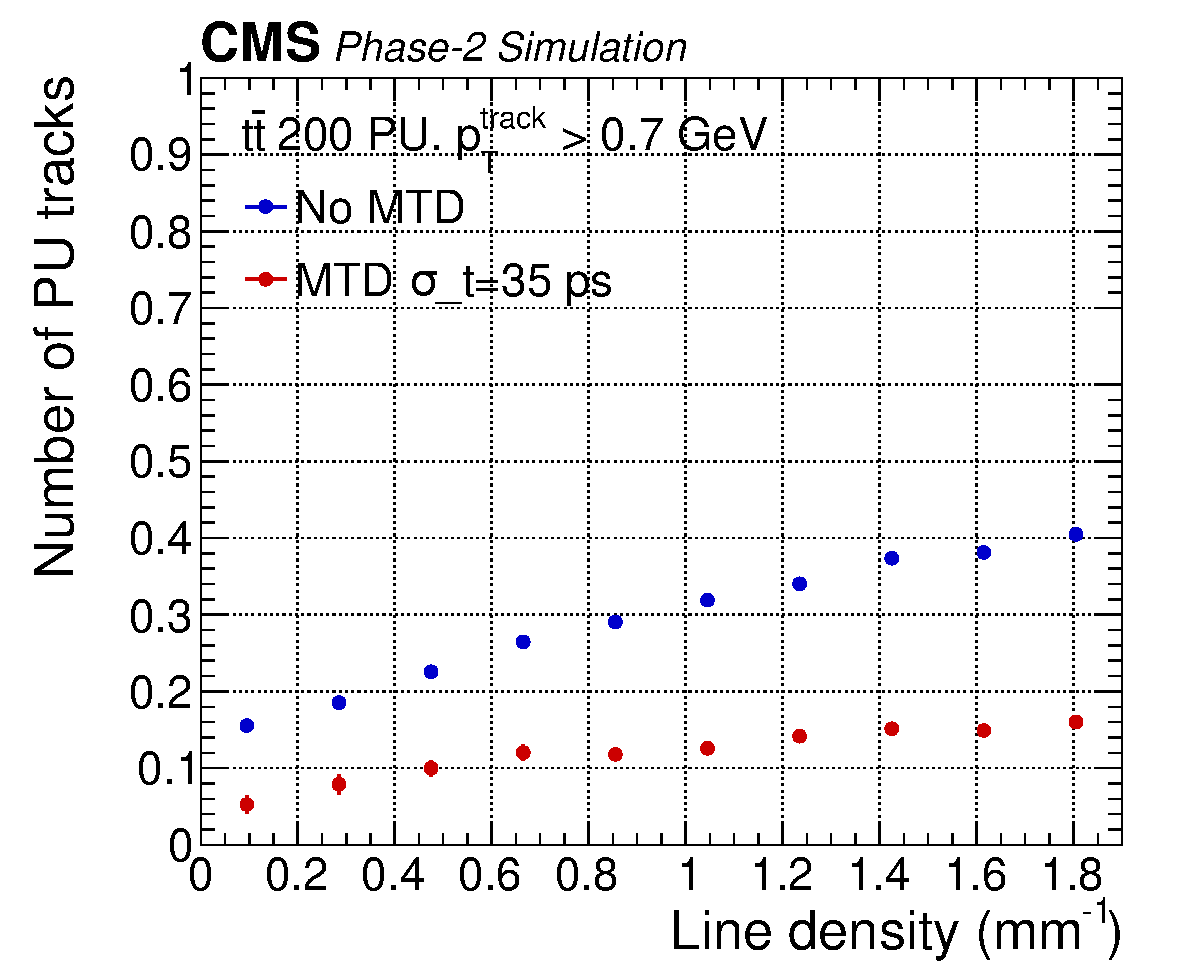
\includegraphics[width=0.52\textwidth]{fig/performance/trkvtx/track_pu_vs_linden_s.pdf}
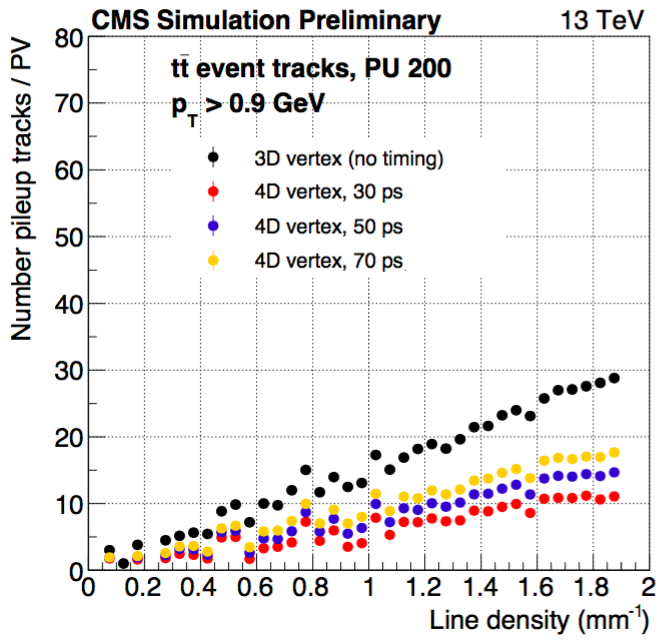
\includegraphics[width=0.44\textwidth]{fig/performance/trkvtx/nPUTracks_fromNtuple_tres.png}
 \caption{Left: Fraction of tracks from pileup incorrectly 
   associated with the hard primary vertex in \ttbar events from full
   simulation as a function of the pileup density, shown with (4D vtx)
   and without (3D vtx) precision timing. Right: Ditto for
   fast-simulation and different assumption on the timing resolution.}
   \label{fig:trkvtx}
\end{figure}
